\chapter{Cloud networking}
\section{Data centers networks}
Unquestionably, networking is the core of \emph{cloud computing}, in fact, it
has been made feasible by the continuous evolution of internet connectivity.
Historically, networks have been classified into three layers:
\begin{itemize}
    \item \emph{Tier 1}: core part of network infrastructure that allows all
    other networks on the internet to communicate each other;
    \item \emph{Tier 2}: portions of \emph{tier 1} infrastructure which is
    bought by internet service providers which then sold access to customers;
    \item \emph{Tier 3}: part of the network infrastructure that allows final
    users to gain access to other networks;
\end{itemize}
\begin{note}
    \emph{Tier 2} networks communicate each other as peers through special nodes
    called Internet Exchange Points (IXP).
\end{note}

\begin{figure}[h!]
    \centering
    \img{network-tiers.png}{0.4}
    \caption{Internet infrastructure}
\end{figure}

\noindent
The transformation of the internet experience, with the shift towards web only
services (e.g. web applications instead of desktop applications), resulted in
a significant increase in volumes of shared data and required bandwidth. To
address this increase in bandwidth demand, cloud providers introduced Content
Delivery Networks (CDN) whose function is to bring service providers closer
to the final users. A secondo step was made with the spread of IoT and
decentralized computing paradigms such as \emph{fog computing}.

\begin{figure}[ht!]
    \centering
    \subfloat[Traditional infrastructure]{\img{traditional-network.png}{0.48}}
    \hfill
    \subfloat[Modern infrastructure]{\img{modern-network.png}{0.48}}\\
    \subfloat[Today's infrastructure]{\img{todays-network.png}{0.48}}\\
\end{figure}

\subsection{Characteristics of data center networks}
Data centers are huge structures with tons of servers, so they demand high
bandwidth with the outside and a very low RTT within their premises. Also,
each data center is a single administrative domain, meaning that its
administrators have full control over its intern network infrastructure, 
endpoints and protocols. This allows them to deviate from standards and adopt
each kind of custom solutions, as long as the services they host are reachable.

This liberty becames relavant as soon as we realize that most of the traffic
in a data center is created by machine-to-machine communications, leaving
user-to-machine traffic a small percentage of the total amount. 

\begin{figure}[h!]
    \centering
    \img{data-center-traffic}{0.5}
    \caption{Traffic within a data center}
\end{figure}

\noindent
This means that performances of networks inside the data centers, which
are called \emph{interconnection networks}, are critical.

\paragraph{Interconnetion networks}
An \emph{interconnection network} is composed of nodes and links, or communication
channels. Nodes can be servers, memory units or even processors. Then, each node
has an interface connecting it to the network, and the number of link the node
is connected defines its degree. The interconnection fabric is made of
switches\footnotemark and links. Switches receive packets, and look inside them
to determine the way toward their final destination. An $n$-way switch is a
switch with $n$ ports that can be connected to $n$ links. The interconnection
fabric determines whether the \emph{interconnection network} is \emph{blocking}
or not. It is \emph{non-blocking} if any permutation of source and destination
nodes can connect each other at any time. It is \emph{blocking} if this is not
true.

\footnotetext{We're refering to a generic switching device without saying if
is a layer 2 or layer 3 one}

\bigskip\noindent
\emph{Interconnection networks} can be distinguished by three parameters:
\begin{itemize}
    \item \emph{Topology}: defines the way nodes are interconnected;
    \item \emph{Routing}: defines how a message gets from source to destination;
    \item \emph{Flow control}: negotiates how the buffer space is allocated;
\end{itemize}
The \emph{topology} also determines the \emph{network diameter} and
\emph{bisection width}.

\begin{definition}[Network diameter]
    Network diameter is defined as the average distance between pairs of
    nodes.
\end{definition}
\begin{definition}[Bisection width]
    Bisection width is defined as the minimum number of links that have to be
    cut to partition the interconnection network into two halves.
\end{definition}

\noindent
When an \emph{interconnection network} is partitioned into two networks of
them same size, the bisection bandwidth measures the communication bandwidth
between the two. We talk about full bisection bandwidth when one half of nodes
can communicate simultaneously with the other half.

\paragraph{Topologies}
There are two main types of \emph{topologies}:
\begin{itemize}
    \item \emph{Static networks}: servers are connected through direct connections;
    \item \emph{Switched networks}: servers are connected through switches;
\end{itemize}

\begin{figure}[h!]
\centering
\subfloat[\emph{Bus topology}]{\resizebox*{0.48\textwidth}{!}{\begin{graph}
    \tikzset{
        rect/.style={rectangle, draw, inner sep=5mm},
    }
    \node[rect] (0) {Memory};
    \node[rect] (1) [right of=0, xshift=20mm] {Memory};
    \node[rect] (2) [right of=1, xshift=20mm] {Memory};
    \node[rect] (3) [right of=2, xshift=20mm] {Memory};

    \node[rect] (4) [below left of=0, yshift=-20mm] {Cache};
    \node[rect] (5) [right of=4, xshift=20mm] {Cache};
    \node[rect] (6) [right of=5, xshift=20mm] {Cache};
    \node[rect] (7) [right of=6, xshift=20mm] {Cache};

    \node[rect] (8) [below of=4, yshift=4.5mm, minimum width=20.9mm,
        minimum height=18mm] {Proc};
    \node[rect] (9) [below of=5, yshift=4.5mm, minimum width=20.9mm,
        minimum height=18mm] {Proc};
    \node[rect] (10) [below of=6, yshift=4.5mm, minimum width=20.9mm,
        minimum height=18mm] {Proc};
    \node[rect] (11) [below of=7, yshift=4.5mm, minimum width=20.9mm,
        minimum height=18mm] {Proc};

    \node[empty] (a) [below of=0, yshift=3mm] {};
    \node[empty] (b) [right of=a, xshift=20mm] {};
    \node[empty] (c) [right of=b, xshift=20mm] {};
    \node[empty] (d) [right of=c, xshift=20mm] {};
    \node[empty] (e) [right of=d, xshift=10mm] {};
    \node[empty] (f) [left of=a, xshift=-10mm] {};
    
    \node[empty] (g) [above of=8, yshift=12.6mm] {};
    \node[empty] (h) [right of=g, xshift=20mm] {};
    \node[empty] (i) [right of=h, xshift=20mm] {};
    \node[empty] (j) [right of=i, xshift=20mm] {};

    \draw[-]    (0) -- (a)
                (1) -- (b)
                (2) -- (c)
                (3) -- (d);

    \draw[-]    (4) -- (g)
                (5) -- (h)
                (6) -- (i)
                (7) -- (j);
    
    \draw[-, line width=1.3pt] (f) -- (e);

    \node[empty] (z) [below of=j, yshift=-45.5mm] {};
\end{graph}}}
\hfill
\subfloat[\emph{Hypercube topology}]{\resizebox*{0.48\textwidth}{!}{\begin{graph}
    \tikzset{
        rect/.style={rectangle, draw, fill, minimum size=3mm, inner sep=0},
        point/.style={circle, draw=gray, fill=gray, minimum size=2mm, inner sep=0},
        every path/.style={draw=gray}
    }
    
    \foreach \x in {0,3}
        \foreach \y in {0,-3}
        {
            \node[point] (a\x\y) at (\x, \y) {};
            \node[rect] (r\x\y) [below right of=a\x\y, shift={(-6mm, 6mm)}] {};
            \node[point] (b\x\y) [below left of=a\x\y, shift={(2mm, 2mm)}] {};
            \node[rect] (r1\x\y) [below right of=b\x\y, shift={(-6mm, 6mm)}] {};

            \draw[-]    (a\x\y) -- (b\x\y)
                        (a\x\y) -- (r\x\y)
                        (b\x\y) -- (r1\x\y);
        }

    \draw[-] (a00) -- (a30) -- (a3-3) -- (a0-3) -- (a00);
    \draw[-] (b00) -- (b30) -- (b3-3) -- (b0-3) -- (b00);

    \foreach \x in {6,9}
        \foreach \y in {0,-3}
        {
            \node[point] (c\x\y) at (\x, \y) {};
            \node[rect] (r2\x\y) [below right of=c\x\y, shift={(-6mm, 6mm)}] {};
            \node[point] (d\x\y) [below left of=c\x\y, shift={(2mm, 2mm)}] {};
            \node[rect] (r3\x\y) [below right of=d\x\y, shift={(-6mm, 6mm)}] {};

            \draw[-]    (c\x\y) -- (d\x\y)
                        (c\x\y) -- (r2\x\y)
                        (d\x\y) -- (r3\x\y);
        }

    \draw[-] (c60) -- (c90) -- (c9-3) -- (c6-3) -- (c60);
    \draw[-] (d60) -- (d90) -- (d9-3) -- (d6-3) -- (d60);
    \draw[-, bend left=25]
        (a00) edge (c60)
        (a30) edge (c90)
        (b00) edge (d60)
        (b30) edge (d90);
    \draw[-, bend right=25]
        (a0-3) edge (c6-3)
        (a3-3) edge (c9-3)
        (b0-3) edge (d6-3)
        (b3-3) edge (d9-3);
\end{graph}}}
\end{figure}
\newpage
\begin{figure}[ht!]
\ContinuedFloat
\centering
\subfloat[\emph{2D-mesh topology}]{\resizebox*{0.48\textwidth}{!}{\begin{graph}
    \tikzset{
        rect/.style={rectangle, draw, fill, minimum size=3mm, inner sep=0},
        point/.style={circle, draw=gray, fill=gray, minimum size=2mm, inner sep=0},
        every path/.style={draw=gray}
    }
    
    \foreach \x in {0, 3, 6, 9}
        \foreach \y in {0,-3, -6, -9}
        {
            \node[point] (a\x\y) at (\x, \y) {};
            \node[rect] (r\x\y) [below right of=a\x\y, shift={(-6mm, 6mm)}] {};

            \draw[-] (a\x\y) -- (r\x\y);
        }

    \foreach \x in {0, 3, 6}
        \foreach \y in {1, ..., 4}
        {
            \FPeval{\res}{clip(\x+3)}
            \ifthenelse{\y = 1}{
                \draw[-] (a\x0) -- (a\res0);
                \draw[-] (a\x0) -- (a\x-3);
            }{
                \ifthenelse{\y = 2}{
                    \draw[-] (a\x-3) -- (a\res-3);
                    \draw[-] (a\x-3) -- (a\x-6);
                }{
                    \ifthenelse{\y = 3}{
                        \draw[-] (a\x-6) -- (a\res-6);
                        \draw[-] (a\x-6) -- (a\x-9);
                    }{
                        \draw[-] (a\x-9) -- (a\res-9);
                    }
                }
            }
        }
    \draw[-]    (a90) -- (a9-3) -- (a9-6) -- (a9-9);
\end{graph}}}
\hfill
\subfloat[\emph{Torus topology}]{\resizebox*{0.48\textwidth}{!}{\begin{graph}
    \tikzset{
        rect/.style={rectangle, draw, fill, minimum size=3mm, inner sep=0},
        point/.style={circle, draw=gray, fill=gray, minimum size=2mm, inner sep=0},
        curve/.style={rounded rectangle, draw, minimum height=15mm,
            minimum width=105mm, shift={(15mm, 7.5mm)}},
        rcurve/.style={rounded rectangle, draw, minimum height=15mm,
            minimum width=105mm, rotate=-90, shift={(15mm, -7.5mm)}},
        every path/.style={draw=gray}
    }
    
    \foreach \x in {0, 3, 6, 9}
        \foreach \y in {0,-3, -6, -9}
        {
            \node[point] (a\x\y) at (\x, \y) {};
            \node[rect] (r\x\y) [below right of=a\x\y, shift={(-6mm, 6mm)}] {};

            \draw[-] (a\x\y) -- (r\x\y);
        }

    \foreach \x in {0, 3, 6}
        \foreach \y in {1, ..., 4}
        {
            \FPeval{\res}{clip(\x+3)}
            \ifthenelse{\y = 1}{
                \draw[-] (a\x0) -- (a\res0);
                \draw[-] (a\x0) -- (a\x-3);
            }{
                \ifthenelse{\y = 2}{
                    \draw[-] (a\x-3) -- (a\res-3);
                    \draw[-] (a\x-3) -- (a\x-6);
                }{
                    \ifthenelse{\y = 3}{
                        \draw[-] (a\x-6) -- (a\res-6);
                        \draw[-] (a\x-6) -- (a\x-9);
                    }{
                        \draw[-] (a\x-9) -- (a\res-9);
                    }
                }
            }
        }
    \draw[-]    (a90) -- (a9-3) -- (a9-6) -- (a9-9);

    \node[curve] (r1) at (a30) {};
    \node[curve] (r2) at (a3-3) {};
    \node[curve] (r3) at (a3-6) {};
    \node[curve] (r4) at (a3-9) {};

    \node[rcurve] (r5) at (a0-3) {};
    \node[rcurve] (r6) at (a3-3) {};
    \node[rcurve] (r7) at (a6-3) {};
    \node[rcurve] (r8) at (a9-3) {};

    \node[empty] (z) [below of=a0-9, yshift=-3.5mm] {};
\end{graph}}}
\caption{\emph{Static networks topologies}}
\end{figure}

\begin{figure}[h!]
    \centering
    \subfloat[\emph{Crossbar switch topology}]{\img{crossbar-switch.png}{0.48}}
    \hfill
    \subfloat[\emph{Omega switch topology}]{\img{omega-switch.png}{0.48}}      
    \caption{\emph{Switched network topologies}}
\end{figure}

\noindent
Up to this point, we can say that an \emph{interconnection network} must be
scalable, provide a high bandwidth with low latency and must guarantee what is
called \emph{location transparent communication}, meaning that every server
should communicate with the others with similar speed and latency. In simple
terms, the position of a server in the data center shouldn't impact
its networking performance. This latter requirement translates in the
impossibility of adopting a hierarchical organization of servers.

Costs also come in hand when designing an \emph{interconnection network}. Both
servers and network apparatus costs are relevant, but talking about networking,
the choice of routers and switches often requires a compromise between latency
and costs. For example, based on the number of ports of a router we can have
low-radix and high-ridix routers. The former has a few ports, while the latter
has more; thus bandwidth is divided into a smaller number of wide ports and
a larger number of narrow ports respectively.

\bigskip\noindent
In general, data centers networks are designed around the following schema:
\begin{figure}[h!]
    \centering
    \img{general-schema.png}{0.6}
    \caption{Generale \emph{interconnetion network} schema}
\end{figure}

\noindent
Layer 2 and layer 3 has pros and cons that have to balanced to guarantee ease
of configuration, administration and problem-solving.

Layer 2, that is the ethernet switching part of the infrastructure, is easy to
configure, thanks to autoconfiguration protocols such as DHCP, and allows the
addition of servers in a plug \& play way, but it's important to limit broadcast
domains to avoid link saturarion due to broadcast frames, and dealing with the
Spanning Tree Protocol might be a struggle.

On the other hand, IP routing on layer 3 makes scalability easy thanks to
hieranchical addressing and allows to obtain multipath routing with equal-cost
multipath\footnote{We will see more about this later in this section}. However,
its configuration is more complex and migration requires changing the IP addresses.

\begin{note}
    At the end of the day, the entire \emph{interconnection network} will look
    like a giant switch that allows all the servers to communicate one another.
\end{note}

\subsection{Topologies more in depth}
In the \emph{butterfly network topology} data always travels through the most
efficient route, but two packets attempting to reach the same port at the same
time would couse a collision, so this is a \emph{blocking topology}.
\begin{note}
    The name comes from the pattern of inverted triangles created by the
    interconnections, which look like butterfly wings.
\end{note}
\emph{Clos networks} is a \emph{non-blocking topology} that consists of two
\emph{butterfly networks} in which the last stage of the output is fused to the
first stage of the output. This way, all packet sent, overshoot their destination
and then hop back to it. However, this overshoot is mostly unnecessary and
increases the latency because each packet takes twice as many hops as it need.
A solution to this is the \emph{folded clos topology} which is obtained by
making input and output nodes share the same switch devices. Such networks are
also called \emph{fat trees} and the \emph{topology} is also called
\emph{fat tree topology}.

\begin{figure}[ht!]
    \centering
    \subfloat[\emph{Clos topology} made of two \emph{3-stage butterfly
    networs} and radix-2 routers]{\img{clos-network.png}{0.48}}
    \hspace{1.5cm}
    \subfloat[\emph{Folded clos topology}]{\img{folded-clos-network.png}{0.3}}
    \caption{\emph{Clos} VS \emph{folded clos topology}}
\end{figure}

\paragraph{Fat tree topology}
In a \emph{fat tree} network, servers are placed at the leafs, while internal
and root nodes are switches. To increase bandwidth, additional links are also
added to near-root nodes. The advantage of such \emph{topology} is that all the
switching elements are identical and this allows costs reductions. Another,
already named, characteristic is the presence of multiple equal-cost path that
both allow for load splitting and \emph{location trasparent communication.}

\begin{figure}[h!]
    \centering
    \img{fat-tree.png}{0.6}
    \caption{Tipical \emph{fat tree topology}}
\end{figure}

\noindent
A \emph{fat tree} made of $k$ pods has two layers and $k/2$ switches for each
pod. Each switch at the lower layer is directly connected to $k/2$ servers
and $k/2$ switches of the upper layer.

\begin{note}
    From the lower to the upper, layers are also called \emph{edge},
    \emph{aggregation} and \emph{core} respectively.
\end{note}

\noindent
Similarly, each \emph{aggregation layer} switch is connected to $k/2$ \emph{core
layer} switches which also have $k/2$ more connections to other aggregation
switches, one for each pod. This configuration results in an infrastructure
that has $4$ servers, actually, $4$ racks with $4$ on-top-of-rack switches,
$k(k+1)$ switches and a total of $(k/2)^2$ paths connecting each pairs of
servers.

When it comes to IP assignment, switches are numbered left-to-right and
bottom-to-top as $base.pod.switch.1$ (in the previous image, $base=87$).
\emph{Core layer} switches instead, are numbered as $base.k.i.j$ where $k$ is
the number of pods and $i,j$ denotates the coordinates of the switch in the
grid, starting from top-left. Finally, servers IPs are in the form
$base.pod.switch.serverID$ and $serverID$ is assigned from left-to-right.

\subsection{Open issues}
Existing \emph{topologies}, including \emph{Fat trees}, still fail to address
workload balancing and TCP-related issues.

\begin{note}
    TCP retransmission and congestiona avoidance policies causes a degradation
    of throughput, so new protocols are currently being developed to displace
    TCP (e.g. QUIC).
\end{note}

\noindent
When it comes to workload, we distinguish between small and large flows. As the
names suggests, the first denotates small flows of data which require low
latency, while the second regards bigger flows which should benefit a higher
throughput.

\begin{note}
    Small and large flows are also called mice and elephants flow respectively.
\end{note}

\begin{eg}[Traffic balancing problems]
Let's assume to be in the following situation and to have many flows going from
$S$ to $D$:

\begin{figure}[h!]
    \centering
    \img{tb-1.png}{0.4}
\end{figure}

\noindent
We want to assign each flow to a path in the most efficient way. We could just
use the Equal-Cost Multipath routing (ECMP) to randomly assign a path to each
flow. This would be a simple approch, but it would also be totally agnostic to
available resources; thus we could experience long-lasting collisions between
elephant flows.

\begin{figure}[h!]
    \centering
    \img{tb-2.png}{0.4}
\end{figure}

\noindent
The problem complicates when we have more source and destination nodes to
connect. Ideally, we would like paths to not intersect each other, like in the
above picture:

\begin{figure}[h!]
    \centering
    \img{tb-3.png}{0.4}
\end{figure}

\noindent
Wrong choices might cause collision in both upward and downward paths:
\begin{figure}[ht!]
    \centering
    \subfloat[Upward path congested]{\img{tb-4.png}{0.4}}
    \hspace{1.5cm}
    \subfloat[Downward path congested]{\img{tb-5.png}{0.4}}
\end{figure}
\end{eg}

\paragraph{Proposed solutions}
Up to now, various solutions have been proposed, but none of them solves complety
all the issues. For example, an idea was to detect elephant flows by putting
a threshold on link capacity (e.g. 10\%), compute non-conflicting path for
each flow over the limit and using plain ECMP for mice flows.

Other proposals where to reroute flows based on link utilization or queue
occupancy. However, the first favors mice flows and, vice versa, the second tends
to promote elephant flows. We could even try to spread all packets evenly, but
that would make congestion control hard to implement.

\section{Networking in virtualised environments}
Virtualization introduces additional complexity for networking, because we need
to deliver traffic between VMs or containers and the outer world and also grant
communication between virtualised environments within the same physical machine.
We also need to decide how to assign IP addresses to VMs and containers and
how to provide advanced features such as load balancing, firewalls, etc.

\begin{note}
    From a networking perspective there is no difference between VMs and
    containers.
\end{note}

\noindent
The first idea would be to imitate what we have in the physical world. So, as
we have many servers connected to a switch who's also connected to a backbone,
in a virtualised environment, we might connect each environment to a virtual
switch and then connect the virtual switch to the physical NIC.

\begin{figure}[h!]
    \centering
    \subfloat[Physical world]{\img{physical-world.png}{0.4}}
    \hspace{1.5cm}
    \subfloat[Virtual world]{\img{virtual-world.png}{0.4}}
    \caption{Copy-paste approch}
\end{figure}

\subsection{North/south and east/west communication on a single server}
Although we suggested that a virtual switch might be the solution to virtual
environments networking, in fact, three main options exists:

\noindent
\begin{minipage}{0.48\textwidth}
\begin{enumerate}
    \item \emph{Host-based switching}: using a virtual switch in the
    \emph{Hypervisor} or directly in the \emph{Host OS};
    \item \emph{NIC switching}: using virtual queues in the NIC;
    \item \emph{Haipin switching}: passing through the external switch;
\end{enumerate}
\end{minipage}
\hfill
\begin{minipage}{0.48\textwidth}
    \centering
    \img{nsew-3-ways.png}{0.48}
\end{minipage}

\paragraph{Host-based switching}
Historically, this is the first solution used and is also called \emph{software
bridge} o \emph{softswitch}.

\bigskip\noindent
\begin{minipage}{0.48\textwidth}
    This solution grants both high bandwidth and reduced overhead for inter-VM
    traffic. Plus, it allows enforcing policies (e.g. firewall rules) directly
    on the virtual switch as if it was a physical one, so the features are the
    same. However, this introduces an additional component to configure (i.e. the
    switch itself has to be configured) and also an additional processing
    overhead because every message has to pass throught said switch.
\end{minipage}
\hfill
\begin{minipage}{0.48\textwidth}
    \centering
    \img{nsew-1.png}{0.48}
\end{minipage}

\bigskip\noindent
It's worth mentioning that this solution requires the physical NIC to operate in
promiscuous mode. That's because, since virtual environments MAC addresses are
different from the physical NIC one and, by default, each NIC doesn't process
packets whose destination MACs are different from its own, those packets would
be dropped.

\paragraph{Hairpin switching}
This solution uses the physical switch, allowing us to leverage its power thus
reducing CPU cycles consumption.

\bigskip\noindent
\begin{minipage}{0.48\textwidth}
    However, this is not necessarily a good thing because PCI bandwidth is
    smaller than CPU-to-Mem bandwidth, thus it might be saturated quickly. Another
    problem is that traffic always need to pass through all the intermediate
    components (e.g. \emph{VMM}, NIC, physical link) and, in case of VM-to-VM
    communications data crosses those components twice. For all of these reasons,
    this solution is no longer used.
\end{minipage}
\begin{minipage}{0.48\textwidth}
    \centering
    \img{nsew-2.png}{0.45}
\end{minipage}

\bigskip\noindent
Again, it's worth mentioning that to use the existing hardware it has to be
compatible with \emph{hairpin switching} because, by default, switches don't
forward traffic on the same port on which it has arrived.

\paragraph{NIC switching}
\emph{NIC switching} is an intermediate solution between the previous two, both
conceptually and in terms of performance.

\bigskip\noindent
\begin{minipage}{0.48\textwidth}
    Again, passing through the NIC means reducing CPU consumption for networkig
    related tasks, but we still have to rely on PIC bandwidth. Since data doesn't
    leave the machine unless it's necessary, we still manage to get improved
    performance in comparison to \emph{hairpin switching}. However, to be able
    to enforce complex or advanced networking policies, a standard NIC might not
    be enught. When that's the case we could opt for a Smart NIC, that is a
    normal NIC with increased computing power.
\end{minipage}
\hfill
\begin{minipage}{0.48\textwidth}
    \centering
    \img{nsew-3.png}{0.48}
\end{minipage}

\bigskip\noindent
Smart NIC are expensive, so their use must be weighed with the characteristics
of the actual infrastructure. For example, if the amount of CPU spent due to
networking tasks is so large that it leaves little or no time left for
applications, it might be worth considering smart NIC adoption. Otherwise, a
\emph{host-based} solution could be enough.

\begin{note}
    For instance, networking may become computationally relevant when using
    overlay tunneling protocol or DDoS detection and prevention algorithms.
\end{note}

\paragraph{Hardware VS software solutions}
Software switches provides better performances when local VM-to-VM traffic is
predominant, but alse when we're dealing with untrusted sources or over-subscribed
links (i.e. tipical cloud service provider situations), or when we need a
fine-grained control over passing data. To get all of this we pay in terms of
CPU consumption reducing resources available to VMs or containers.

Hardware switches instead, are good when most of the traffic is between different
servers and when we're applying similar policies to all nodes in the data center.
Currently, software solutions are the most used.

\section{Software bridges in Linux}
Linux allows creating a bridge across many interfaces and one unique virtual
interface that is valid for the entire host.

\begin{figure}[h!]
    \centering
    \subfloat{\img{traditional-network-2.png}{0.4}}
    \hspace{1.5cm}
    \subfloat{\img{bridged-network.png}{0.4}}
    \caption{Traditional VS bridged network}
\end{figure}

\noindent
In the past, the setup of a bridging process in Linux was a way to have an 802.1D
bridge, running in software, that was part of a bigger network, thus allowing
us to modify the bridge code and play with it without having to buy a physical
device. Now, it became a way to overcome the limitations of the IP protocol who
requires each interface to have a unique address. Linux offers three ways to
create a software bridge: \emph{Linuxbridge}, \emph{macvlan} and \emph{Open
vSwitch}.

\subsection{Linuxbridge}
This is the most common kind of bridge, and it behaves exactly like a physical
one. To receive packets intended for virtual hosts, it requires NICs to work in
promiscuous mode. In fact, packets intended for virtual hosts will have the MAC
address of \texttt{br0} virtual device as destination. Then, traffic can be
sent from both physical and virtual interfaces and the IP address configured in
the bridge is reachable from both interfaces (i.e. it works like a sort of
loopback address).

\subsection{Macvlan}
\emph{Macvlan} implements a VLAN-like behaviour by using MAC addresses instead
of 802.1Q tags. Each virtual environment can be assigned to a differenct
\emph{macvlan interface}, and each interface has its own MAC address and a
distinc IP. \emph{Macvlan} supports four operating modes: \emph{private},
\emph{VEPA}, \emph{bridge} and \emph{pass-through}. For all of these, except
for the latter, supporting NIC can be configured to filter unicast packets
based on their MAC address instead of running in promiscuous mode.

\paragraph{Private mode}
\emph{Macvlan} in \emph{private mode} mimics exactly the behaviour of VLANs,
meaning that \emph{inter-macvlan} traffic is forbidden and different
\emph{macvlans} can communicate only by passing through a router.

\paragraph{VEPA mode}
In the case of \emph{VEPA mode}, which stands for \emph{Virtual Ethernet Port
Aggregator}, $A$ and $B$ can't communicate directly each other, instead, they
need to send their frames to a physical switch out of the server (actually, it
may also be a layer 2 switch on the NIC), and when the frame is sent back into
the server, the \emph{macvlan} drivers can deliver the data correctly.

\begin{figure}[hb!]
    \centering
    \subfloat[\emph{Macvlan} overview]{\img{macvlan-1.png}{0.24}}
    \hspace{1.5cm}
    \subfloat[\emph{Macvlan private mode}]{\img{macvlan-private.png}{0.24}}
    \hspace{1.5cm}
    \subfloat[\emph{Macvlan VEPA mode}]{\img{macvlan-vepa.png}{0.24}}
\end{figure}
\newpage
\begin{figure}[h!]
    \ContinuedFloat
    \centering
    \subfloat[\emph{Macvlan bridge mode}]{\img{macvlan-bridge.png}{0.24}}
    \hspace{1.5cm}
    \subfloat[\emph{Macvlan pass-through mode}]{\img{macvlan-pass-through.png}{0.24}}
    \caption{\emph{Macvlan} modes}
\end{figure}

\noindent
The problem is that the external switch can't be a traditional 802.1D bridge, for
the same reason we've already talked about: switches don't sent data back to
the same port on which it was received. However, \emph{VEPA mode} is the default
one.

\paragraph{Bridge mode}
\emph{Bridge mode} emulates a simple bridge, that is a bridge with just one
uplink, no filtering database (i.e. no MAC learning) and no Spanning Tree
Protocol. By means of that, it can forward all kind of traffic, without
necessarily going out of the server and then back into it.

\paragraph{Pass-through mode}
This mode supports only one \emph{macvlan} device, that is to say it can handle
a single VM, for instance. This way, all traffic can be sent to the upstream
component (e.g. the traffic can be sent directly to a VM), and said component
can use any MAC address because, nor the \emph{macvlan} drivers, now the NIC
do any MAC filtering; it will be the VM virtual NIC who will take charge of that.
In fact, MAC $A$ is no longer used. Of cource the physical NIC needs to work in
promiscuous mode.

\begin{note}
    \emph{Pass-through mode} behaves like if the physical NIC were directly
    assigned to the virtual environment.
\end{note}

\paragraph{Linuxbridge VS macvlan}
\emph{Linuxbridge} drivers behaves as a traditional hardware bridge, so they can
handle complex situations in which, for instance, hosts on the same physical
domain (layer 2 network) resides both on the same host and outside it. They're
also useful when more VMs or containers on the same host need to communicate,
or when advanced functions (e.g. flood control) are needed.

\emph{Macvlan} drivers instead, are both simpler and less CPU consuming, because
they emulate a trivial bridge with basic functionalities. Therefore, they're
recommended when you just need to provide egress connection to the physical
network to virtual machines or containers.

\subsection{Open vSwitch}
\emph{Open vSwitch} (\emph{OVS}) is a software implementation of a virtual
multilayer network switch, designed to enable effective network automation
through programmatic extensions. It can operate both as a software-based network
switch running within a \emph{VMM} and a control stack for dedicated switching
hardware. Talking about its implementation, it is implemente into the Linux
Kernel, and it's designed to support both standard management interfaces and
protocols (e.g. NetFlow, sFlow, \dots) and transparent distribution across
multiple physical servers by enabling creation of cross-server switches in a way
that abstracts out the underlying server architecture.

\begin{note}
    \emph{Open vSwitch} is often implemented into cloud computing software
    platforms and virtualization management systems (e.g. OpenStack, OpenNebula).
\end{note}

\begin{figure}[h!]
    \centering
    \img{ovs.png}{1}
    \caption{\emph{Open vSwitch} general implementation schema}
\end{figure}

\section{Single server networking services}
\paragraph{IP assignment}
The first problem is about deciding who should assign IP addresses to VMs and
containers and also which addresses should be assigned. The first option could
be to use the same addresses of the physical (meaning non virtualised) network
so that inboud and outbound connections toward VMs or containers don't differe.
However, this approch would require the coordination of the physical network
manager, thus limiting virtualization agility.

The alternative, would be to use private addresses and then connect to the
internet through a NAT. This would be good because IP assignment wouldn't
be limited by public IP limits, and it wouldn't require coordination with the
physical network manager. Of course, we would have to define static rules to
support inbound connectivity and virtual environment would be reached by
different IP addresses depending on wheter the sender is inside or outside the
private network.

\begin{note}
    The first solution proposed is also called \emph{direct routing}.
\end{note}

\newpage
\begin{figure}[ht!]
    \centering
    \subfloat[\emph{Direct routing}]{\img{ip-problem-1.png}{0.38}}
    \hspace{2cm}
    \subfloat[\emph{NATted routing}]{\img{ip-problem-2.png}{0.2}}
    \caption{Solutions to IP assignent}
\end{figure}

\paragraph{Providing feature-rich network connectivity}
Up to this point it should be clear that providing additional network services
may require connecting VMs or containers to the physical infrastructure. For
example, if private IPs are used for VMs, the \emph{hypervisor} must also provide
a router, NAT and a DHCP service. To do this, we can exploit functionalities
provided either by the kernel or by another software such as Docker engine o
similar. For example, we can handle NAT tables using the \texttt{iptables} tool.

\paragraph{Multi-tenancy}
Accomplishing \emph{multi-tenancy}, that is to say, accomplishing a strong network
isolation, is a must in virtualised environments.

\begin{figure}[h!]
    \centering
    \img{multi-tenancy.png}{0.4}
    \caption{\emph{Multi-tenancy}}
\end{figure}

\noindent
In the physical world this can be achieved through VLANs. However, in a server
it's much more convenient to just create multiple virtual switches and
routers.

\paragraph{Tenant-defined network services}
Each tenant might require a complex topology. For example a tenent might deploy
3 VMs who can communicate each other, but just one of which can access the
internet. Again, we can achieve this by simply using pre-defined functionalities,
provided either by the kernel or by other pieces of software.

\begin{figure}[ht!]
    \centering
    \img{tenant-defined-network-services.png}{0.3}
    \caption{\emph{Tenant-defined network services}}
\end{figure}

\paragraph{Co-existence of virtual services and host applications}
Up to now we didn't mention that host servers have their own TCP/IP stacks, and
they need to co-exist together with all the other virtualised services.

\begin{figure}[h!]
    \centering
    \img{virtual-and-host-services.png}{0.3}
    \caption{Virtual and host services co-existence}
\end{figure}

\noindent
In particular, there should be a way to distinguish between traffic directed towards
host applications and VMs or containers. To do so we can exploit the Linux
networking stack.

\paragraph{Putting all together}
Putting all together what we've said so far, we obtain the following general schema:

\begin{figure}[h!]
    \centering
    \img{putting-all-together1.png}{0.40}
    \caption{Putting all together}
\end{figure}

\noindent
So, virtual routers and virtual NAT services are in fact implemented into the
Linux networking stack. Each cluster of VMs or containers is associated to a
virtual NIC. Each virtual environment has its own MAC address and so the virtual
NIC. In what we've called \emph{NATted mode}, all frames sent by hosts with
a virtual MAC, passed through the kernel IP stack who translated those addresses
according to pre-defined NAT rules. Then, inbound traffic follows the same route
backward up to its destination.

\begin{eg}[Example of communication]
    Let's consider a packet sent by VM1 to the internet:

    \begin{figure}[h!]
        \centering
        \subfloat{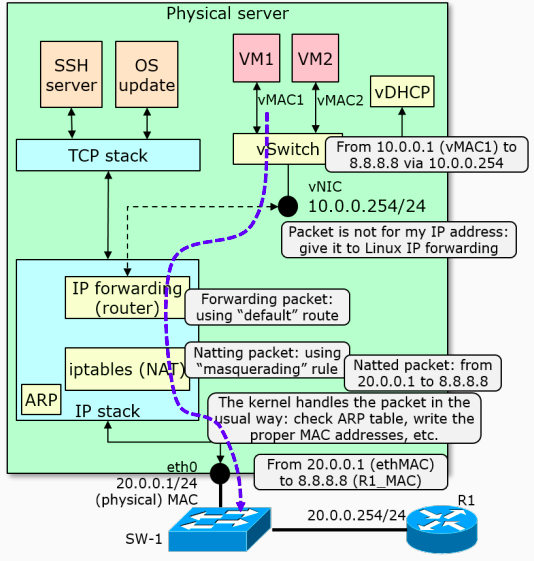
\includegraphics[width=0.48\textwidth, valign=c]{putting-all-together-details.png}}
        \hfill
        \subfloat{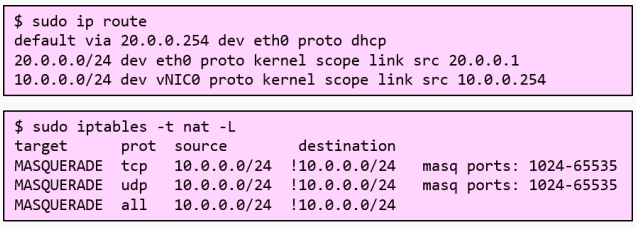
\includegraphics[width=0.48\textwidth, valign=c]{putting-all-together-tables.png}}
    \end{figure}

    \noindent
    So, VM1 sends the packet to its default gateway, which is \texttt{vNIC}. 
    The vNIC receives the packet, it detects that it is not the final recipient,
    so the packet is transferred to the Linux IP forwarding module. Finally,
    the Linux IP forwarding module forwards the packet to the next hop based on
    the host routing and NAT tables as usual
\end{eg}

\section{Data center-wide networking services}
When moving from a single server to a data center we need to solve the same
problem as before. First of all, we have to distinguish between \emph{tenant}
and \emph{cloud manager view}. The first wants to deploy some services without
caring about the underlying physical infrastructure. The cloud manager instead
has to manage the physical infrastructure so that it's able to provide the
requested logical view.

\subsection{Providing layer 2 connectivity}
Tenents may want to have a vannilla layer 2 connectivity that spans amongs all of
its services across the data center. This is the case in which tenants want to
take IP addressing under their own responsibility. The solution to this kind of
request is the creation of tunnels between servers. What we'll see are tunnels
managed by GRE (General Router Encapsulation).

\newpage
\begin{figure}[ht!]
    \centering
    \img{layer2.png}{0.8}
    \caption{Characteristics required by layer 2 connectivity}
\end{figure}

\begin{figure}[h!]
    \centering
    \subfloat[\emph{Tenent view}]{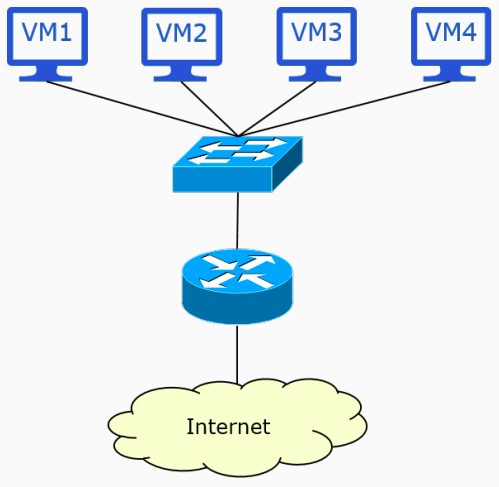
\includegraphics[width=0.38\textwidth, valign=c]{t-view1.png}}
    \hspace{1.5cm}
    \subfloat[\emph{Cloud manager view}]{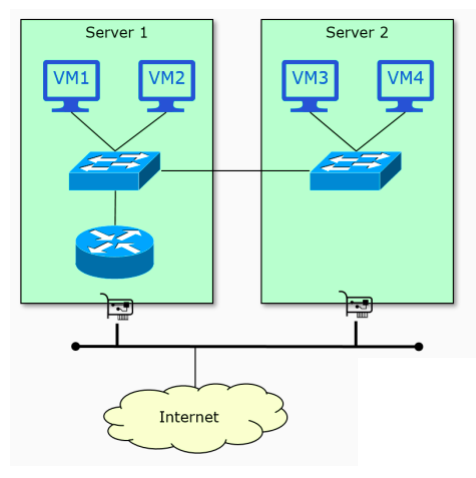
\includegraphics[width=0.38\textwidth, valign=c]{cm-view1.png}}
    \caption{\emph{Tenenat} VS \emph{cloud manager view}}
\end{figure}

\begin{eg}[Example of communication]
    Let's consider a packet sent by VM2 to VM3:

    \begin{figure}[h!]
        \centering
        \img{tunneling-l2-1.png}{0.8}
    \end{figure}

    \noindent
    To provide layer 2 connectivity between virtual machines on two different
    physical servers we have created a tunnel (i.e. the red dotted line between
    two virtual NICs). Essentially, what happens is that, when the packet sent
    by VM2 reaches the virtual switch, it forwards the packed to \texttt{vTUN0}
    device. \texttt{vTUN0} is the interface associated with the tunnel and its
    remote IP tells what is the IP to which that packet has to be sent. In this
    case it is \texttt{3.0.0.1}, which is the address of the second physical
    server, beacause VM3 resides in it. So, the tunneling protocol wraps the
    original packet with a new IP packet that has destination address
    \texttt{3.0.0.1} and source \texttt{2.0.0.1} which is the address of physical
    server 1. The packet is finally taken by the Linux networking stack which
    sends the packet.

    The destination server, receives the packet, sends it to the tunnel
    device, which decapsulates the additional headers and finally forwars the
    original frame to the correct destination.
\end{eg}
\begin{note}
    In this situation NAT isn't necessary because the resulting packet looks
    like a packet sent by an host application.
\end{note}

\noindent
Could we have used VLAN instead of tunnels?

Short answer: no. The reason is that it would require cooperation with the
physical network manager. Also, VLANs are limited to 4096 and setting up
everything would be trickier than what we've done for tunnels.

\subsection{Providing layer 3 connectivity}
With layer 3 connectivity, tenants rely on a cloud service provider for IP
assignment and management, and this can be achieved in two ways:
\emph{tunneling} and \emph{direct routing}.

\begin{figure}[h!]
    \centering
    \img{layer3.png}{0.8}
    \caption{Characteristics required by layer 3 connectivity}
\end{figure}

\begin{eg}[Example of communication using tunnels]
    Let's consider the same case as before: a packet sent by VM2 to VM3:

    \begin{figure}[h!]
        \centering
        \img{layer3-t-details-1.png}{0.8}
    \end{figure}

    \noindent
    This time the tunnel interface is connected to the Linux virtual router. Once
    the packet reaches that interface it is again encapsulated into the same
    packet as before, and then sent back to the router who forwards it outside
    and up to the other server.

    \newpage
    \begin{figure}[ht!]
        \centering
        \img{layer3-t-details-2.png}{0.8}
    \end{figure}

    \noindent
    Once the packet has reached the destination server and has arrived to the other
    side of the tunnel, the original packet is decapsulated and sent up to VM3.
\end{eg}
\begin{note}
    VM2 and VM3 are on different private networks.
\end{note}

\begin{eg}[Example of communication using direct routing]
    Let's consider the same situation as before, but with direct routing instead
    of tunneling:

    \begin{figure}[h!]
        \centering
        \img{layer-3-dr-1.png}{0.8}
    \end{figure}

    \noindent
    This time, the packet is sent directly out of the server without any
    modifications, and it reaches router \texttt{R1}. The router knows, because
    it has been configured, that the destination network \texttt{10.0.2.0/24}
    (i.e. the network to which VM3 is connected) is reachable via \texttt{30.0.0.0/24}
    network. So, the packet is forwarded out of the interface with IP
    \texttt{30.0.0.254} with next hop address set to \texttt{30.0.0.1}, that is
    the address of the second physical server.

    \bigskip\noindent
    When the packet reaches the destination server, it can go directly up to
    VM3 as a normal packet.

    \newpage
    \begin{figure}[ht!]
        \centering
        \img{layer-3-dr-2.png}{0.8}
    \end{figure}
\end{eg}

\begin{note}
    It's easy to understand the route of every packet if the behaviour of every
    component is considered alone.
\end{note}
\begin{note}
    Even if we've proceded in our discussion considering inconvinient any
    solution that required to manage directly physical hardware, \emph{layer 3
    connectivity} through \emph{direct routing} is often used, and is made
    convenient by the possibility to configure routers via a set of REST APIs.
\end{note}

\paragraph{Tunnels in practice}
For the sake of semplcity we've considered a single tunnel between a pair of
servers, but this is obviously difficult to handle on a large scale because
it would require a full mesh of connections. This is therefore the reason for
which tunneling technologies such as GRE (Generic Routing Encapsulation) are
often replaced by others. In particular, \emph{VxLAN} allows providing both a
trasparent full mesh solution, with a single endpoint for all the hosts
belonging to the same VxLAN domain, and a way of distributing traffic across
multiple parallel links through layer 4 ports.

\begin{figure}[h!]
    \centering
    \img{layer-4.png}{0.5}
    \caption{\emph{VxLAN network}}
\end{figure}

\paragraph{Tunneling VS direct routing}
\emph{Tunneling} enables the deployment of tenant services without any
interaction with the infrastructure provider and becomes useful in case of
public datacenters. However, it may trigger some performance problems due to
the reduced MTU on the tunnel: since packets are being encpasulated, the maximum
size of the original packets must be reduced. \emph{Direct routing} on the other
hand, doesn't require changing the MTU, but the infrastructure provider has to
cooperate.